%package list
\documentclass{article}
\usepackage[top=3cm, bottom=3cm, outer=3cm, inner=3cm]{geometry}
\usepackage{multicol}
\usepackage{graphicx}
\usepackage{url}
%\usepackage{cite}
\usepackage{hyperref}
\usepackage{array}
%\usepackage{multicol}
\newcolumntype{x}[1]{>{\centering\arraybackslash\hspace{0pt}}p{#1}}
\usepackage{natbib}
\usepackage{pdfpages}
\usepackage{multirow}
\usepackage[normalem]{ulem}
\useunder{\uline}{\ul}{}
\usepackage{svg}
\usepackage{xcolor}
\usepackage{listings}
\lstdefinestyle{ascii-tree}{
    literate={├}{|}1 {─}{--}1 {└}{+}1 
  }
\lstset{basicstyle=\ttfamily,
  showstringspaces=false,
  commentstyle=\color{red},
  keywordstyle=\color{blue}
}
%\usepackage{booktabs}
\usepackage{caption}
\usepackage{subcaption}
\usepackage{float}
\usepackage{array}

\newcolumntype{M}[1]{>{\centering\arraybackslash}m{#1}}
\newcolumntype{N}{@{}m{0pt}@{}}


%%%%%%%%%%%%%%%%%%%%%%%%%%%%%%%%%%%%%%%%%%%%%%%%%%%%%%%%%%%%%%%%%%%%%%%%%%%%
%%%%%%%%%%%%%%%%%%%%%%%%%%%%%%%%%%%%%%%%%%%%%%%%%%%%%%%%%%%%%%%%%%%%%%%%%%%%
\newcommand{\itemEmail}{vmamanian@unsa.edu.pe}
\newcommand{\itemStudent}{Victor Mamani Anahua}
\newcommand{\itemCourse}{Fundamentos de la Programación II}
\newcommand{\itemCourseCode}{20230489}
\newcommand{\itemSemester}{II}
\newcommand{\itemUniversity}{Universidad Nacional de San Agustín de Arequipa}
\newcommand{\itemFaculty}{Facultad de Ingeniería de Producción y Servicios}
\newcommand{\itemDepartment}{Departamento Académico de Ingeniería de Sistemas e Informática}
\newcommand{\itemSchool}{Escuela Profesional de Ingeniería de Sistemas}
\newcommand{\itemAcademic}{2023 - B}
\newcommand{\itemInput}{Del 25 Octubre 2023}
\newcommand{\itemOutput}{Al 1 Noviembre 2023}
\newcommand{\itemPracticeNumber}{09}
\newcommand{\itemTheme}{Laboratorio 09}
%%%%%%%%%%%%%%%%%%%%%%%%%%%%%%%%%%%%%%%%%%%%%%%%%%%%%%%%%%%%%%%%%%%%%%%%%%%%
%%%%%%%%%%%%%%%%%%%%%%%%%%%%%%%%%%%%%%%%%%%%%%%%%%%%%%%%%%%%%%%%%%%%%%%%%%%%

\usepackage[english,spanish]{babel}
\usepackage[utf8]{inputenc}
\AtBeginDocument{\selectlanguage{spanish}}
\renewcommand{\figurename}{Figura}
\renewcommand{\refname}{Referencias}
\renewcommand{\tablename}{Tabla} %esto no funciona cuando se usa babel
\AtBeginDocument{%
	\renewcommand\tablename{Tabla}
}

\usepackage{fancyhdr}
\pagestyle{fancy}
\fancyhf{}
\setlength{\headheight}{30pt}
\renewcommand{\headrulewidth}{1pt}
\renewcommand{\footrulewidth}{1pt}
\fancyhead[L]{\raisebox{-0.2\height}{
\includegraphics[width=3cm]{img/logo_episunsa.png}}}
\fancyhead[C]{\fontsize{7}{7}\selectfont	\itemUniversity \\ \itemFaculty \\ \itemDepartment \\ \itemSchool \\ \textbf{\itemCourse}}
\fancyhead[R]{\raisebox{-0.2\height}{
\includegraphics[width=1.2cm]{img/logo_abet}}}
\fancyfoot[L]{Estudiante Victor Mamani A.}
\fancyfoot[C]{\itemCourse}
\fancyfoot[R]{Página \thepage}

% para el codigo fuente
\usepackage{listings}
\usepackage{color, colortbl}
\definecolor{dkgreen}{rgb}{0,0.6,0}
\definecolor{gray}{rgb}{0.5,0.5,0.5}
\definecolor{mauve}{rgb}{0.58,0,0.82}
\definecolor{codebackground}{rgb}{0.95, 0.95, 0.92}
\definecolor{tablebackground}{rgb}{0.8, 0, 0}

\lstdefinestyle{java}{frame=tb,
	language=Java,
	showstringspaces=false,
	columns=flexible,
	basicstyle={\footnotesize\ttfamily\color[RGB]{255,255,255}},
	numberstyle=\color{mygray},
	numbers=left, 
	keywordstyle=\color{myblue},
	morekeywords={String, System},
	commentstyle=\color{mygray},
	stringstyle=\color{mygreen},
	breaklines=true,
	breakatwhitespace=true,
	tabsize=2,
	backgroundcolor= \color{codebackgroundCode},
	showspaces=false,
	showtabs=false,
	showlines=false,
}

\lstset{frame=tb,
	language=bash,
	aboveskip=3mm,
	belowskip=3mm,
	showstringspaces=false,
	columns=flexible,
	basicstyle={\small\ttfamily},
	numbers=none,
	numberstyle=\tiny\color{gray},
	keywordstyle=\color{blue},
	commentstyle=\color{dkgreen},
	stringstyle=\color{mauve},
	breaklines=true,
	breakatwhitespace=true,
	tabsize=3,
	backgroundcolor= \color{codebackground},
}

\begin{document}
	
	\vspace*{10px}
	
	\begin{center}	
		\fontsize{17}{17} \textbf{ Informe de Laboratorio \itemPracticeNumber}
	\end{center}
	\centerline{\textbf{\Large Tema: \itemTheme}}
	%\vspace*{0.5cm}	

	\begin{flushright}
		\begin{tabular}{|M{2.5cm}|N|}
			\hline 
			\rowcolor{tablebackground}
			\color{white} \textbf{Nota}  \\
			\hline 
			     \\[30pt]
			\hline 			
		\end{tabular}
	\end{flushright}	

	\begin{table}[H]
		\begin{tabular}{|x{4.7cm}|x{4.8cm}|x{4.8cm}|}
			\hline 
			\rowcolor{tablebackground}
			\color{white} \textbf{Estudiante} & \color{white}\textbf{Escuela}  & \color{white}\textbf{Asignatura}   \\
			\hline 
			{\itemStudent \par \itemEmail} & \itemSchool & {\itemCourse \par Semestre: \itemSemester \par Código: \itemCourseCode}     \\
			\hline 			
		\end{tabular}
	\end{table}		
	
	\begin{table}[H]
		\begin{tabular}{|x{4.7cm}|x{4.8cm}|x{4.8cm}|}
			\hline 
			\rowcolor{tablebackground}
			\color{white}\textbf{Laboratorio} & \color{white}\textbf{Tema}  & \color{white}\textbf{Duración}   \\
			\hline 
			\itemPracticeNumber & \itemTheme & 04 horas   \\
			\hline 
		\end{tabular}
	\end{table}
	
	\begin{table}[H]
		\begin{tabular}{|x{4.7cm}|x{4.8cm}|x{4.8cm}|}
			\hline 
			\rowcolor{tablebackground}
			\color{white}\textbf{Semestre académico} & \color{white}\textbf{Fecha de inicio}  & \color{white}\textbf{Fecha de entrega}   \\
			\hline 
			\itemAcademic & \itemInput &  \itemOutput  \\
			\hline 
		\end{tabular}
	\end{table}
	
	\section{Tarea}
	\begin{itemize}		
        \item Cree un Proyecto llamado Laboratorio9
        \item Crear 3 constructores sobrecargados.
        \item La actitud puede ser defensiva, ofensiva, fuga. Dicha actitud varía cuando el soldado defiende, ataca o huye respectivamente.
        \item Al atacar el soldado avanza, al avanzar aumenta su velocidad en 1. Al defender el soldado se para. Al huir aumenta su velocidad en 2. Al retroceder, si su velocidad es mayor que 0, entonces primero para y su actitud es defensiva, y si su velocidad es 0 entonces disminuirá a valores negativos. Al ser atacado su vida actual disminuye y puede llegar incluso a morir.
        \item Crear los atributos y métodos extra que considere necesarios.
		\item Usted deberá crear las dos clases Soldado.java y VideoJuego5.java. Puede reutilizar lo desarrollado en Laboratorios anteriores.
		\item Del Soldado nos importa el nombre, puntos de vida, fila y columna (posición en el tablero).
		\item El juego se desarrollará en el mismo tablero de los laboratorios anteriores. Para el tablero utilizar la estructura de datos más adecuada.
		\item Tendrá 2 Ejércitos. Inicializar el tablero con n soldados aleatorios entre 1 y 10 para cada Ejército. Cada soldado tendrá un nombre autogenerado: Soldado0X1, Soldado1X1, etc., un valor de puntos de vida autogenerado aleatoriamente [1..5], la fila y columna también autogenerados aleatoriamente (no puede haber 2 soldados en el mismo cuadrado). 
		\item Además de los datos del Soldado con mayor vida de cada ejército, el promedio de puntos de vida de todos los soldados creados por ejército, los datos de todos los soldados porejército en el orden que fueron creados y un ranking de poder de todos los soldados creados por ejército (del que tiene más nivel de vida al que tiene menos) usando 2 diferentes algoritmos de ordenamiento (indicar conclusiones respecto a este ordenamiento de HashMaps).
		\item Finalmente, que muestre qué ejército ganará la batalla (indicar la métrica usada para decidir al ganador de la batalla).
		\item Crear el diagrama de clases UML.
	\end{itemize}

	\section{Equipos, materiales y temas utilizados}
	\begin{itemize}
		\item Sistema Operativo Ubuntu GNU Linux 23 lunar 64 bits Kernell 6.2.v
		\item Visual Studio Code.
		\item VIM 9.0.
		\item OpenJDK 64-Bits 19.0.7.
		\item Git 2.39.2.
		\item Cuenta en GitHub con el correo institucional.
		\item Programación Orientada a Objetos.
		\item Actividades del Laboratorio 08.	
	\end{itemize}
	
	\section{URL de Repositorio Github}
	\begin{itemize}
		\item URL del Repositorio GitHub para clonar o recuperar.
		\item \url{https://github.com/VictorMA18/fp2-23b.git}
		\item URL para el laboratorio 09 en el Repositorio GitHub.
		\item \url{https://github.com/VictorMA18/fp2-23b/tree/main/Fase02/Lab09}
	\end{itemize}
	
	\section{Actividades del Laboratorio 09}

	\subsection{Ejercicio Soldado}
	\begin{itemize}	
		\item En el primer commit reutilizamos la clase Soldado de los anteriores laboratorios el cual a este le quitamos el atributo health y lo cambiamos con lifealctual y tambien añadimos diferentes atributos y diferentes metodos añadimos el 2do constructor el cual este me da un objeto nulo el cual lo podremos utilizar para poder reemplazar las casillas en blanco y tambien en el otro constructor le ponemos ya sus atributos correspondientes el cual este soldado va a tener.
		\item El codigo y el commit seria el siguiente:
	\end{itemize}	
	\begin{lstlisting}[language=bash,caption={Commit}][H]
		$ git commit -m "Completando los atributos del constructor de la clase Soldado() el cual este va a ser para cuando el objeto sea nulo"
	\end{lstlisting}	
	\begin{lstlisting}[language=java,caption={Las lineas de codigos del metodo creado:}][H]
		// Laboratorio Nro 9  - Ejercicio Soldado
		// Autor: Mamani Anahua Victor Narciso
		// Colaboro:
		// Tiempo:
		import java.util.*;
		public class Soldado { //CREAMOS LA CLASE SOLDODADO PARA PODER USAR UN ARREGLO BIDIMENSIONAL DONDE NECESITAMOS LA VIDA , EL NOMBRE DEL SOLDADO Y TAMBIEN SU POSICION COMO LA FILA Y LA COLUMNA   
		
			private String name;
			private int health;
			private int row;
			private String column;
			private int attacklevel;
			private int defenselevel;
			private int lifelevel;
			private int lifeactual;
			private int speed;
			private String attitude;
			private boolean lives;
		
			Random rdm = new Random();
		
			//Anadiendo metodo que nos permita que un arreglo tenga datos nulos si este esta vacio
			public Soldado(){
				this.name = "";
				this.health = 0;
				this.row = 0;
				this.column  = "";
				this.attacklevel = 0;
				this.defenselevel = 0;
				this.lifelevel = 0;
				this.lifeactual = 0;
				this.speed = 0;
				this.attitude = "";
				this.lives = false;
			}
		
			//Constructor
			public Soldado(String name, int health, int row, String column){
				this.name = name;
				this.health = health;
				this.lifeactual = health;
				this.row = row;
				this.column = column;
				this.lives = true;
		
				//YA QUE ESTOS DATOS SERIAN ALEATORIOS YA QUE SE ESTARIA CREANDO EL SOLDADO TENDRIAMOS DATOS QUE SERIAN COMO ATTACKLEVEL DEFENSELEVEL EL CUAL TENDRIAN QUE SER ALEATORIOS    
				this.attacklevel = rdm.nextInt(5) + 1;
				this.defenselevel = rdm.nextInt(5) + 1;
		
			}
		
			//Constructor para los diferentes niveles como de vidad defensa ataque velocidad
		
			// Metodos mutadores
			public void setName(String n){
				name = n;
			}
			public void setHealth(int p){
				health = p;
			}
			public void setRow(int b){
				row = b;
			}
			public void setColumn(String c){
				column = c; 
			}
		
			// Metodos accesores
			public String getName(){
				return name;
			}
			public int getHealth(){
				return health;
		
			}
			public int getRow(){
				return row;
			}
			public String getColumn(){
				return column;
			}
		
			// Completar con otros metodos necesarios
			public String toString(){ //CREAMOS ESTE METODO PARA IMPRIMIR LOS DATOS DEl OBJETO
				String join = "\nNombre: " + getName() + "\nVida: " + getHealth() + "\nFila: " + getRow() + "\nColumna: " + getColumn(); //Agregamos un espaciador para poder separar
				return join;
			}
		}

	\end{lstlisting}
	\subsection{Ejercicio Soldado}
	\begin{itemize}	
		\item En el segundo commit creamos el 3er constructor el cual tendremos los niveles la velocidad y su estado tambien añadimos sus getters y setters , tambien modificamos el metodo toString() el cual nos dara toda la informacion del soldado
		\item El codigo y el commit seria el siguiente:
	\end{itemize}	
	\begin{lstlisting}[language=bash,caption={Commit}][H]
		$ git commit -m "Creamos el 3er constructor el cual tendremos los niveles la velocidad y su estado tambien anadimos sus getters y setters , tambien modificamos el metodo toString() el cual nos dara toda la informacion del soldado"
	\end{lstlisting}	
	\begin{lstlisting}[language=java,caption={Las lineas de codigos del metodo creado:}][H]
		public Soldado(String name , int attacklevel, int defenselevel, int lifelevel, int speed, boolean lives, int row, String column) {
			this.name = name;
			this.attacklevel = attacklevel;
			this.defenselevel = defenselevel;
			this.lifelevel = lifelevel;
			this.speed = speed;
			this.lives = lives;
			this.row = row;
			this.column = column;
		}
		public void setAttackLevel(int attacklevel) {
			this.attacklevel = attacklevel;
		}
		public void setDefenseLevel(int defenselevel) {
			this.defenselevel = defenselevel;
		}
		public void setLifeLevel(int lifelevel){
			this.lifelevel = lifelevel;
		}
		public void setSpeed(int speed) {
			this.speed = speed;
		}
		public void setAttitude(String attitude) {
			this.attitude = attitude;
		}
		public void setLives(boolean lives) {
			this.lives = lives;
		}

		public int getAttackLevel() {
			return attacklevel;
		}
		public int getDefenseLevel() {
			return defenselevel;
		}
		public int getLifeLevel(){
			return lifelevel;
		}
		public int getSpeed() {
			return speed;
		}
		public String getAttitude() {
			return attitude;
		}
		public boolean getLives() {
			return lives;
		}
		public String toString(){ //CREAMOS ESTE METODO PARA IMPRIMIR LOS DATOS DEl OBJETO
			String join = "\nNombre: " + getName() + "\nVida: " + getLifeActual() + "\nFila: " + getRow() + "\nColumna: " + getColumn() + "\nNivel de ataque: " + getAttackLevel() + "\nNivel de Defensa: " + getDefenseLevel() + "\nNivel de vida: " + getLifeLevel() + "\nVelocidad: " + getSpeed() + "\nActitud: " + getAttitude() + "\nEstado: " + getLives(); //Agregamos un espaciador para poder separar
        	return join;
    	}

	\end{lstlisting}
	\subsection{Ejercicio Soldado}
	\begin{itemize}	
		\item En el tercer commit añadimos los metodos restantes a los cuales se les podra identificar debido al mensaje que estos daran y saber la accion que estan ejecutando por ejemplo como advance() defense() flee() back() attaack() metodos pedidos que se hagan para los soldados
		\item El codigo y el commit seria el siguiente:
	\end{itemize}	
	\begin{lstlisting}[language=bash,caption={Commit}][H]
		$ git commit -m "Anadiendo los metodos restantes a los cuales se les podra identificar debido al mensaje que estos daran y saber la accion que estan ejecutando por ejemplo como advance() defense() flee() back() attaack() metodos pedidos que se hagan para los soldados"
	\end{lstlisting}	
	\begin{lstlisting}[language=java,caption={Las lineas de codigos del metodo creado:}][H]
		public void defense(){
			this.speed = 0;
			this.attitude = "DEFENSIVA";
			System.out.println("El soldado " + this.name + "esta defendiendo");
		}
		public void flee(){
			this.speed = getSpeed() + 2;
			this.attitude = "HUYE";
			System.out.println("El soldado " + this.name + "esta huyendo");
		}
		public void back(){
			System.out.println("El soldado " + this.name + "esta retrocediendo");
			if(this.speed == 0){
				this.speed = rdm.nextInt(5) - 5;
			}else{
				if(this.speed > 0){
					this.speed = 0;
					this.attitude = "DEFENSIVA";
				}
			}
		}
		public void attaack(Soldado soldier){
			if(this.getLifeActual() > soldier.getLifeActual()){
				int life = this.getLifeActual() - soldier.getLifeActual();
				this.setLifeActual(life);
				this.setLifeLevel(life);
				soldier.lives = false;
				System.out.println(this.name + " asesino al soldado " + soldier.name);
			}else if(soldier.getLifeActual() > this.getLifeActual()){
				int life = soldier.getLifeActual() - this.getLifeActual();
				this.lives = false;
				soldier.setLifeActual(life);
				soldier.setLifeLevel(life);
				System.out.println(soldier.name + " asesino al soldado " + this.name);
			}else{
				this.lives = false;
				soldier.lives = false;
				System.out.println("los 2 soldados se asesinaron");
			}
		}

	\end{lstlisting}
	\subsection{Ejercicio Videojuego}
	\begin{itemize}	
		\item En el cuarto commit creamos el metodo fillRegister() el cual nos ayudara a poder registar a soldados los cuales van a ser creados el cual tambien en este comprobamos que 2 soldados del mismo ejercito no se repitan para esto creamos una condicional ala vez hicimos pruebas para poder saber si lo puesto como condiciones exista cuando lo imprimamos esto de final de este metodo nos retornara a los soldados creados de cada ejercito por orden de creacion el cual va a ser sus datos
		\item El codigo , el commit y la ejecución seria el siguiente:
	\end{itemize}	
	\begin{lstlisting}[language=bash,caption={Commit}][H]
		$ git commit -m "Creando el metodo fillRegister() el cual nos ayudara a poder registar a soldados los cuales van a ser creados el cual tambien en este comprobamos que 2 soldados del mismo ejercito no se repitan para esto creamos una condicional ala vez hicimos pruebas para poder saber si lo puesto como condiciones exista cuando lo imprimamos esto de final de este metodo nos retornara a los soldados creados de cada ejercito por orden de creacion el cual va a ser sus datos"
	\end{lstlisting}	
	\begin{lstlisting}[language=java,caption={Las lineas de codigos del metodo creado:}][H]
		import java.util.*;
		class Videojuego { 
			public static ArrayList<ArrayList<Soldado>> fillRegister(int num){
				Random rdm = new Random();
				ArrayList<ArrayList<Soldado>> army = new ArrayList<ArrayList<Soldado>>();
				int numbersoldiers = rdm.nextInt(10) + 1; //NUMERO DE SOLDADOS ALEATORIOS ENTRE 1 A 10 SOLDADOS 
				for(int i = 0; i < 10; i++){ //ITERACION
					army.add(new ArrayList<Soldado>()); //LLENAMOS NUESTROS ARRAYLIST BIDIMENSIONAL CON CADA FILA PARA QUE CUMPLAN CON ESTRUCTURA DEL TABLERO
					for(int j = 0; j < 10 ; j++){//ITERACION
						army.get(i).add(null); // LLENAMOS CADA FILA DEL ARRAYLIST CON UN OBJETO SOLDADO CON TAL QUE ESTE SEA NULL PARA QUE SEPA QUE ESTE TIENE UNA CASILLA PERO NO HAY NADIE TODAVIA SE PUEDE LLENAR 
					}
				}
				System.out.println("El Ejercito " + num + " tiene " + numbersoldiers + " soldados : " ); 
				System.out.println("");
				for(int i = 0; i < numbersoldiers; i++){ //LLENAMOS CASILLAS CON CADA SOLDADO CREADO ALEATORIAMENTE
					String name = "Soldado" + i + "X" + num;
					//System.out.println(name); PRUEBA QUE SE HIZO PARA VER LOS NOMBRES
					int health = rdm.nextInt(5) + 1;
					int row = rdm.nextInt(10) + 1;
					int speed = rdm.nextInt(5) + 1;
					String column = String.valueOf((char)(rdm.nextInt(10) + 65)); //REUTILIZAMOS CODIGO DEL ANTERIOR ARCHIVO VIDEOJUEGO2.JAVA YA QUE TENDRIAN LA MISMA FUNCIONALIDAD
					//System.out.println(army.get(row - 1).get((int)column.charAt(0) - 65)); PRUEBA QUE SE HIZO PARA COMPROBAR SI EL OBJETO SE ESTABA DANDO O NO CAPAZ NI EXISTIA  
					if(army.get(row - 1).get((int)column.charAt(0) - 65) == null){
						System.out.print("Registrando al " + (i + 1) + " soldado del Ejercito " + num + "");
						army.get(row - 1).set((int)column.charAt(0) - 65, new Soldado(name, health, row, column));
						army.get(row - 1).get((int)column.charAt(0) - 65).setSpeed(speed);
						System.out.println(army.get(row - 1).get((int)column.charAt(0) - 65).toString());
						System.out.println("---------------------------------");
					}else{
						i -= 1; //NOS AYUDARIA CON LOS SOLDADOS QUE SE REPITEN EN EL MISMO CASILLERO CON TAL QUE NO DEBERIA CONTAR 
					}
				}
				System.out.println("*********************************");
				return army;
			}
			public static void main(String args[]){
				ArrayList<ArrayList<Soldado>> army1 = fillRegister(1);
				ArrayList<ArrayList<Soldado>> army2 = fillRegister(2);
			}
		}

	\end{lstlisting}
	\begin{lstlisting}[language=bash,caption={Ejecucion:}][H]
		El Ejercito 1 tiene 9 soldados : 

		Registrando al 1 soldado del Ejercito 1
		Nombre: Soldado0X1
		Vida: 1
		Fila: 5
		Columna: C
		Nivel de ataque: 2
		Nivel de Defensa: 1
		Nivel de vida: 1
		Velocidad: 1
		Actitud: null
		Estado: true
		---------------------------------
		Registrando al 2 soldado del Ejercito 1
		Nombre: Soldado1X1
		Vida: 2
		Fila: 6
		Columna: B
		Nivel de ataque: 4
		Nivel de Defensa: 4
		Nivel de vida: 2
		Velocidad: 2
		Actitud: null
		Estado: true
		---------------------------------
		Registrando al 3 soldado del Ejercito 1
		Nombre: Soldado2X1
		Vida: 5
		Fila: 3
		Columna: J
		Nivel de ataque: 1
		Nivel de Defensa: 1
		Nivel de vida: 5
		Velocidad: 5
		Actitud: null
		Estado: true
		---------------------------------
		Registrando al 4 soldado del Ejercito 1
		Nombre: Soldado3X1
		Vida: 2
		Fila: 3
		Columna: B
		Nivel de ataque: 3
		Nivel de Defensa: 4
		Nivel de vida: 2
		Velocidad: 2
		Actitud: null
		Estado: true
		---------------------------------
		Registrando al 5 soldado del Ejercito 1
		Nombre: Soldado4X1
		Vida: 3
		Fila: 9
		Columna: G
		Nivel de ataque: 2
		Nivel de Defensa: 4
		Nivel de vida: 3
		Velocidad: 3
		Actitud: null
		Estado: true
		---------------------------------
		Registrando al 6 soldado del Ejercito 1
		Nombre: Soldado5X1
		Vida: 1
		Fila: 9
		Columna: J
		Nivel de ataque: 5
		Nivel de Defensa: 4
		Nivel de vida: 1
		Velocidad: 3
		Actitud: null
		Estado: true
		---------------------------------
		Registrando al 7 soldado del Ejercito 1
		Nombre: Soldado6X1
		Vida: 5
		Fila: 4
		Columna: F
		Nivel de ataque: 3
		Nivel de Defensa: 4
		Nivel de vida: 5
		Velocidad: 4
		Actitud: null
		Estado: true
		---------------------------------
		Registrando al 8 soldado del Ejercito 1
		Nombre: Soldado7X1
		Vida: 4
		Fila: 4
		Columna: H
		Nivel de ataque: 3
		Nivel de Defensa: 3
		Nivel de vida: 4
		Velocidad: 1
		Actitud: null
		Estado: true
		---------------------------------
		Registrando al 9 soldado del Ejercito 1
		Nombre: Soldado8X1
		Vida: 5
		Fila: 3
		Columna: H
		Nivel de ataque: 3
		Nivel de Defensa: 4
		Nivel de vida: 5
		Velocidad: 5
		Actitud: null
		Estado: true
		---------------------------------
		*********************************
		El Ejercito 2 tiene 3 soldados : 
		
		Registrando al 1 soldado del Ejercito 2
		Nombre: Soldado0X2
		Vida: 3
		Fila: 6
		Columna: G
		Nivel de ataque: 2
		Nivel de Defensa: 2
		Nivel de vida: 3
		Velocidad: 2
		Actitud: null
		Estado: true
		---------------------------------
		Registrando al 2 soldado del Ejercito 2
		Nombre: Soldado1X2
		Vida: 5
		Fila: 3
		Columna: E
		Nivel de ataque: 5
		Nivel de Defensa: 3
		Nivel de vida: 5
		Velocidad: 4
		Actitud: null
		Estado: true
		---------------------------------
		Registrando al 3 soldado del Ejercito 2
		Nombre: Soldado2X2
		Vida: 5
		Fila: 1
		Columna: B
		Nivel de ataque: 5
		Nivel de Defensa: 2
		Nivel de vida: 5
		Velocidad: 4
		Actitud: null
		Estado: true
		---------------------------------
		*********************************
		
	\end{lstlisting}	
	\subsection{Ejercicio Videojuego}
	\begin{itemize}	
		\item En el quinto commit creamos el metodo viewBoard() el cual nos va a poder imprimir el tablero en donde se va a poder reconocer los soldados de cada ejercito para esto tendriamos que hacer una comparacion de que soldado esta mas fuerte por reclamar su casillero el cual si uno de estos es mas fuerto este se va poder quedar con el casillero en caso de que los 2 sean igual de fuertes en vida entonces los 2 moririan para esto se tuvo que hacer ciertas condiciones al final de esto nos dara la tabla la cual esta va a ser graficada
		\item El codigo , el commit y la ejecución seria el siguiente:
	\end{itemize}	
	\begin{lstlisting}[language=bash,caption={Commit}][H]
		$ git commit -m "Creamos el metodo viewBoard() el cual nos va a poder imprimir el tablero en donde se va a poder reconocer los soldados de cada ejercito para esto tendriamos que hacer una comparacion de que soldado esta mas fuerte por reclamar su casillero el cual si uno de estos es mas fuerto este se va poder quedar con el casillero en caso de que los 2 sean igual de fuertes en vida entonces los 2 moririan para esto se tuvo que hacer ciertas condiciones al final de esto nos dara la tabla la cual esta va a ser graficada"
	\end{lstlisting}	
	\begin{lstlisting}[language=java,caption={Las lineas de codigos del metodo creado:}][H]
		public static void viewBoard(ArrayList<ArrayList<Soldado>> army1, ArrayList<ArrayList<Soldado>> army2){ //EN ESTE METODO DEMOSTRAREMOS LA TABLA REUTILIZAREMOS CODIGOS DE ANTERIORES LABORATORIOS PARA PODER HACER LA BASE DE ESTE TABLERO
			System.out.println("\nMostrando tabla de posicion ... --");
			System.out.println("Leyenda: Ejercito1 --> X | Ejercito2 --> Y"); //RECONOCIMIENTO PARA LOS EJERCITOS Y POSICION DE SUS SOLDADOS
			System.out.println("\n \t   A\t   B\t   C\t   D\t   E\t   F\t   G\t   H\t   I\t   J"); // RECONOCIMIENTO PARA CADA UBICACION DE CADA SOLDADO EN EL TABLERO POR PARTE DE LAS COLUMNAS
			System.out.println("\t_________________________________________________________________________________");
			for(int i = 0; i < 10; i++ ){
				System.out.print((i + 1) + "\t"); // RECONOCIMIENTO PARA CADA UBICACION DE CADA SOLDADO EN EL TABLERO POR PARTE DE LAS FILAS
					for(int j = 0; j < 10; j++){
							if(army1.get(i).get(j) != null && army2.get(i).get(j) != null){ //CREAMOS UN IF PARA QUE ESTE NOS AYUDE A SABER QUIEN DE ESTOS SOLDADOS SE OCUPARA DEL CASILLERO EL CUAL DONDE ESTAN PELEANDO
								if(army1.get(i).get(j).getLifeActual() > army2.get(i).get(j).getLifeActual()){
									army1.get(i).get(j).setLifeActual(army1.get(i).get(j).getLifeActual() - army2.get(i).get(j).getLifeActual()); //Cambiamos 
									army2.get(i).set(j, null); 
									System.out.print("|   " + "X" + "   ");
								}else if(army2.get(i).get(j).getLifeActual() > army1.get(i).get(j).getLifeActual()){
									army2.get(i).get(j).setLifeActual(army2.get(i).get(j).getLifeActual() - army1.get(i).get(j).getLifeActual());
									army1.get(i).set(j, null);;
									System.out.print("|   " + "Y" + "   ");
								}else{
									army2.get(i).set(j, null);
									army1.get(i).set(j, null);
									System.out.print("|   " + " " + "   ");
								}
							}else if(army1.get(i).get(j) != null){
								System.out.print("|   " + "X" + "   ");
							}else if(army2.get(i).get(j) != null){
								System.out.print("|   " + "Y" + "   ");
							}else{
								System.out.print("|   " + " " + "   ");
							}
					}
					System.out.println("|");
					System.out.println("\t|_______|_______|_______|_______|_______|_______|_______|_______|_______|_______|");
			}
			System.out.println("\n*********************************");

		}

	\end{lstlisting}
	\begin{lstlisting}[language=bash,caption={Ejecucion:}][H]
		El Ejercito 1 tiene 8 soldados : 

		Registrando al 1 soldado del Ejercito 1
		
		Nombre: Soldado0X1
		Vida: 4
		Fila: 7
		Columna: J
		Nivel de ataque: 1
		Nivel de Defensa: 5
		Nivel de vida: 4
		Velocidad: 2
		Actitud: null
		Estado: true
		---------------------------------
		Registrando al 2 soldado del Ejercito 1
		
		Nombre: Soldado1X1
		Vida: 4
		Fila: 9
		Columna: J
		Nivel de ataque: 1
		Nivel de Defensa: 4
		Nivel de vida: 4
		Velocidad: 5
		Actitud: null
		Estado: true
		---------------------------------
		Registrando al 3 soldado del Ejercito 1
		
		Nombre: Soldado2X1
		Vida: 4
		Fila: 7
		Columna: F
		Nivel de ataque: 5
		Nivel de Defensa: 1
		Nivel de vida: 4
		Velocidad: 3
		Actitud: null
		Estado: true
		---------------------------------
		Registrando al 4 soldado del Ejercito 1
		
		Nombre: Soldado3X1
		Vida: 1
		Fila: 9
		Columna: B
		Nivel de ataque: 2
		Nivel de Defensa: 4
		Nivel de vida: 1
		Velocidad: 1
		Actitud: null
		Estado: true
		---------------------------------
		Registrando al 5 soldado del Ejercito 1
		
		Nombre: Soldado4X1
		Vida: 2
		Fila: 8
		Columna: G
		Nivel de ataque: 5
		Nivel de Defensa: 5
		Nivel de vida: 2
		Velocidad: 1
		Actitud: null
		Estado: true
		---------------------------------
		Registrando al 6 soldado del Ejercito 1
		
		Nombre: Soldado5X1
		Vida: 3
		Fila: 2
		Columna: C
		Nivel de ataque: 5
		Nivel de Defensa: 2
		Nivel de vida: 3
		Velocidad: 4
		Actitud: null
		Estado: true
		---------------------------------
		Registrando al 7 soldado del Ejercito 1
		
		Nombre: Soldado6X1
		Vida: 2
		Fila: 6
		Columna: E
		Nivel de ataque: 3
		Nivel de Defensa: 3
		Nivel de vida: 2
		Velocidad: 5
		Actitud: null
		Estado: true
		---------------------------------
		Registrando al 8 soldado del Ejercito 1
		
		Nombre: Soldado7X1
		Vida: 5
		Fila: 7
		Columna: I
		Nivel de ataque: 4
		Nivel de Defensa: 2
		Nivel de vida: 5
		Velocidad: 4
		Actitud: null
		Estado: true
		---------------------------------
		*********************************
		El Ejercito 2 tiene 6 soldados : 
		
		Registrando al 1 soldado del Ejercito 2
		
		Nombre: Soldado0X2
		Vida: 2
		Fila: 8
		Columna: I
		Nivel de ataque: 4
		Nivel de Defensa: 3
		Nivel de vida: 2
		Velocidad: 3
		Actitud: null
		Estado: true
		---------------------------------
		Registrando al 2 soldado del Ejercito 2
		
		Nombre: Soldado1X2
		Vida: 3
		Fila: 2
		Columna: D
		Nivel de ataque: 4
		Nivel de Defensa: 1
		Nivel de vida: 3
		Velocidad: 3
		Actitud: null
		Estado: true
		---------------------------------
		Registrando al 3 soldado del Ejercito 2
		
		Nombre: Soldado2X2
		Vida: 4
		Fila: 5
		Columna: G
		Nivel de ataque: 5
		Nivel de Defensa: 5
		Nivel de vida: 4
		Velocidad: 3
		Actitud: null
		Estado: true
		---------------------------------
		Registrando al 4 soldado del Ejercito 2
		
		Nombre: Soldado3X2
		Vida: 3
		Fila: 10
		Columna: A
		Nivel de ataque: 3
		Nivel de Defensa: 2
		Nivel de vida: 3
		Velocidad: 2
		Actitud: null
		Estado: true
		---------------------------------
		Registrando al 5 soldado del Ejercito 2
		
		Nombre: Soldado4X2
		Vida: 5
		Fila: 5
		Columna: A
		Nivel de ataque: 1
		Nivel de Defensa: 5
		Nivel de vida: 5
		Velocidad: 3
		Actitud: null
		Estado: true
		---------------------------------
		Registrando al 6 soldado del Ejercito 2
		
		Nombre: Soldado5X2
		Vida: 4
		Fila: 5
		Columna: C
		Nivel de ataque: 2
		Nivel de Defensa: 5
		Nivel de vida: 4
		Velocidad: 2
		Actitud: null
		Estado: true
		---------------------------------
		*********************************
		
		Mostrando tabla de posicion ... --
		Leyenda: Ejercito1 --> X | Ejercito2 --> Y
		
	\end{lstlisting}
	\begin{figure}[H]
		\centering
		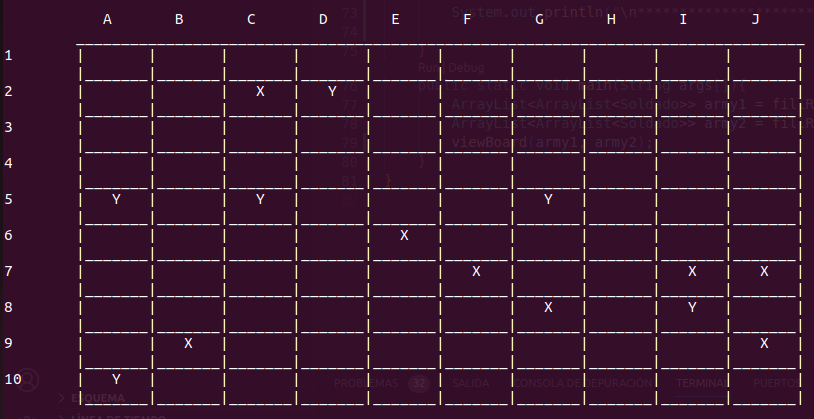
\includegraphics[width=1.0\textwidth,keepaspectratio]{img/Commit5.png}
		%\includesvg{img/automata.svg}
		%\label{img:mot2}
		%\caption{Product backlog.}
	\end{figure}
	\subsection{Estructura de laboratorio 09}
	\begin{itemize}	
		\item El contenido que se entrega en este laboratorio09 es el siguiente:
	\end{itemize}
	\begin{lstlisting}[style=ascii-tree]
	/Lab09	
		"Poner RAMA"

	\end{lstlisting}    
	\section{\textcolor{red}{Rúbricas}}
	
	\subsection{\textcolor{red}{Entregable Informe}}
	\begin{table}[H]
		\caption{Tipo de Informe}
		\setlength{\tabcolsep}{0.5em} % for the horizontal padding
		{\renewcommand{\arraystretch}{1.5}% for the vertical padding
		\begin{tabular}{|p{3cm}|p{12cm}|}
			\hline
			\multicolumn{2}{|c|}{\textbf{\textcolor{red}{Informe}}}  \\
			\hline 
			\textbf{\textcolor{red}{Latex}} & \textcolor{blue}{El informe está en formato PDF desde Latex,  con un formato limpio (buena presentación) y facil de leer.}   \\ 
			\hline 
			
			
		\end{tabular}
	}
	\end{table}
	
	\clearpage
	
	\subsection{\textcolor{red}{Rúbrica para el contenido del Informe y demostración}}
	\begin{itemize}			
		\item El alumno debe marcar o dejar en blanco en celdas de la columna \textbf{Checklist} si cumplio con el ítem correspondiente.
		\item Si un alumno supera la fecha de entrega,  su calificación será sobre la nota mínima aprobada, siempre y cuando cumpla con todos lo items.
		\item El alumno debe autocalificarse en la columna \textbf{Estudiante} de acuerdo a la siguiente tabla:
	
		\begin{table}[ht]
			\caption{Niveles de desempeño}
			\begin{center}
			\begin{tabular}{ccccc}
    			\hline
    			 & \multicolumn{4}{c}{Nivel}\\
    			\cline{1-5}
    			\textbf{Puntos} & Insatisfactorio 25\%& En Proceso 50\% & Satisfactorio 75\% & Sobresaliente 100\%\\
    			\textbf{2.0}&0.5&1.0&1.5&2.0\\
    			\textbf{4.0}&1.0&2.0&3.0&4.0\\
    		\hline
			\end{tabular}
		\end{center}
	\end{table}	
	
	\end{itemize}
	
	\begin{table}[H]
		\caption{Rúbrica para contenido del Informe y demostración}
		\setlength{\tabcolsep}{0.5em} % for the horizontal padding
		{\renewcommand{\arraystretch}{1.5}% for the vertical padding
		%\begin{center}
		\begin{tabular}{|p{2.7cm}|p{7cm}|x{1.3cm}|p{1.2cm}|p{1.5cm}|p{1.1cm}|}
			\hline
    		\multicolumn{2}{|c|}{Contenido y demostración} & Puntos & Checklist & Estudiante & Profesor\\
			\hline
			\textbf{1. GitHub} & Hay enlace URL activo del directorio para el  laboratorio hacia su repositorio GitHub con código fuente terminado y fácil de revisar. &2 &X &2 & \\ 
			\hline
			\textbf{2. Commits} &  Hay capturas de pantalla de los commits más importantes con sus explicaciones detalladas. (El profesor puede preguntar para refrendar calificación). &4 &X &4 & \\ 
			\hline 
			\textbf{3. Código fuente} &  Hay porciones de código fuente importantes con numeración y explicaciones detalladas de sus funciones. &2 &X &2 & \\ 
			\hline 
			\textbf{4. Ejecución} & Se incluyen ejecuciones/pruebas del código fuente  explicadas gradualmente. &2 &X &2 & \\ 
			\hline			
			\textbf{5. Pregunta} & Se responde con completitud a la pregunta formulada en la tarea.  (El profesor puede preguntar para refrendar calificación).  &2 &X &2 & \\ 
			\hline	
			\textbf{6. Fechas} & Las fechas de modificación del código fuente estan dentro de los plazos de fecha de entrega establecidos. &2 &X &2 & \\ 
			\hline 
			\textbf{7. Ortografía} & El documento no muestra errores ortográficos. &2 &X &2 & \\ 
			\hline 
			\textbf{8. Madurez} & El Informe muestra de manera general una evolución de la madurez del código fuente,  explicaciones puntuales pero precisas y un acabado impecable.   (El profesor puede preguntar para refrendar calificación).  &4 &X &2 & \\ 
			\hline
			\multicolumn{2}{|c|}{\textbf{Total}} &20 & &18 & \\ 
			\hline
		\end{tabular}
		%\end{center}
		%\label{tab:multicol}
		}
	\end{table}
	
\clearpage

\section{Referencias}
\begin{itemize}			
	\item \url{https://drive.google.com/file/d/1TbYqdgt7cGTuw_P_ZnkiAXBmPI8YhDMb/view}
\end{itemize}	
	
%\clearpage
%\bibliographystyle{apalike}
%\bibliographystyle{IEEEtranN}
%\bibliography{bibliography}
			
\end{document}